\FloatBarrier
\subsection{LetterLizardJS: JavaScript Letter Lizard Implementation}
\label{lljs}

JavaScript is the ``language of the Web'' and has become an indispensable 
tool for Web developers. Client-side JavaScript scripts executed in Web
browsers are able to bring life to Web pages by interacting with the user,
controlling the behaviour of the browser, performing asynchronous communication
with Web servers and altering the document that is displayed. Although originally
introduced by Netscape for client-side scripting in 1995, it is increasingly
more common for JavaScript to be used in other contexts as well. For example,
a recent trend has been to implement server-side applications in JavaScript as
has been demonstrated by the explosion in popularity of Node.js~\cite{nodejs} and other
server-side JavaScript frameworks. Not long after Netscape started shipping 
JavaScript in its Navigator browser, it submitted the language to Ecma International
and it is now standardized as ECMA-262 and known as ECMAScript.
There are several well-known implementations of the language that conform to the standard.

JavaScript is a dynamic, prototype-based object-oriented language with first-class
functions. Much of its syntax has been influenced by C, C++ and Java, but
its semantics are actually very different. JavaScript borrows key design principles
from Self and Scheme. JavaScript supports several different programming
paradigms including object-oriented, imperative, and functional. JavaScript supports
structured programming similar to C with many of the same flow-control statements
such as \texttt{if}, \texttt{for}, \texttt{while}, etc. One notable difference,
however, is the lack of block scoping for variables. Instead, JavaScript 
uses function scoping for variables, which means that all variable declared in a
function are visible throughout the entire body of the function. 
JavaScript also contains a mechanism that tries to
correct faulty programs by automatically inserting semicolons to complete statements, but quite
often this masks more serious errors~\cite{goodparts} or results in unexpected behaviour.
We explore these issues further in sections~\ref{varscope} and~\ref{lexstruct} respectively.

JavaScript has a dynamic type system in which types are associated with values,
not variables. A few primitive types are provided by the language, such
as Number, String, Boolean, null and undefined. Aside from the primitive types,
everything else is an Object. Objects are composite types
that are comprised of properties: name-value pairs where the name is a String
(or an integer for arrays, we will see more about this in section~\ref{objects})
and the value is one of the primitive types or another object. Even functions
are objects (with associated behaviour), which means that functions are first-class
entities that may be assigned to variables and returned from other functions.

Each JavaScript function also contain a reference to the scope chain that was
in effect when the function was defined, which is used to resolve variable
names to values when the function is executed. A function, together with a
reference to its scope chain is know as a \emph{closure} (we will cover closures
in section~\ref{closures}). 
JavaScript usually runs in event-driven environments, such as the client-side
environment of a Web browser, that make heavy use of closures and first-class 
functions for callbacks.

JavaScript supports object-oriented programming, but not in the classical
sense. Rather than providing class-based inheritance, JavaScript provides
\emph{prototype-based inheritance}. We discuss object-oriented programming
in section~\ref{oop}.

\begin{figure}
    \centering
    \begin{subfigure}{0.49\textwidth}
        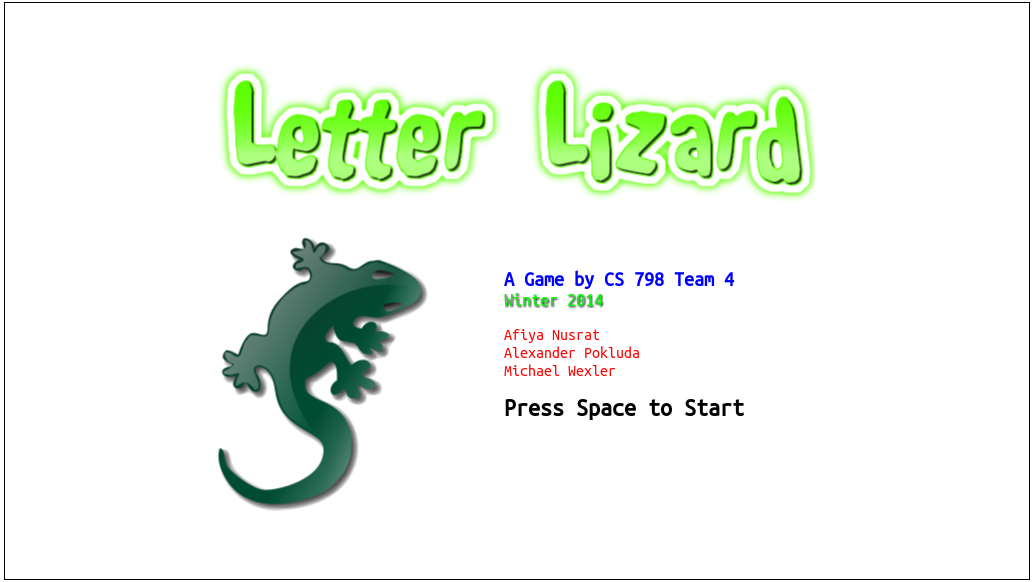
\includegraphics[width=0.9\textwidth]{../screenshots/LetterLizardJS-SplashScreen2.png}
        \caption{Splash Screen}
        \label{lljssplash}
    \end{subfigure}
    \begin{subfigure}{0.49\textwidth}
        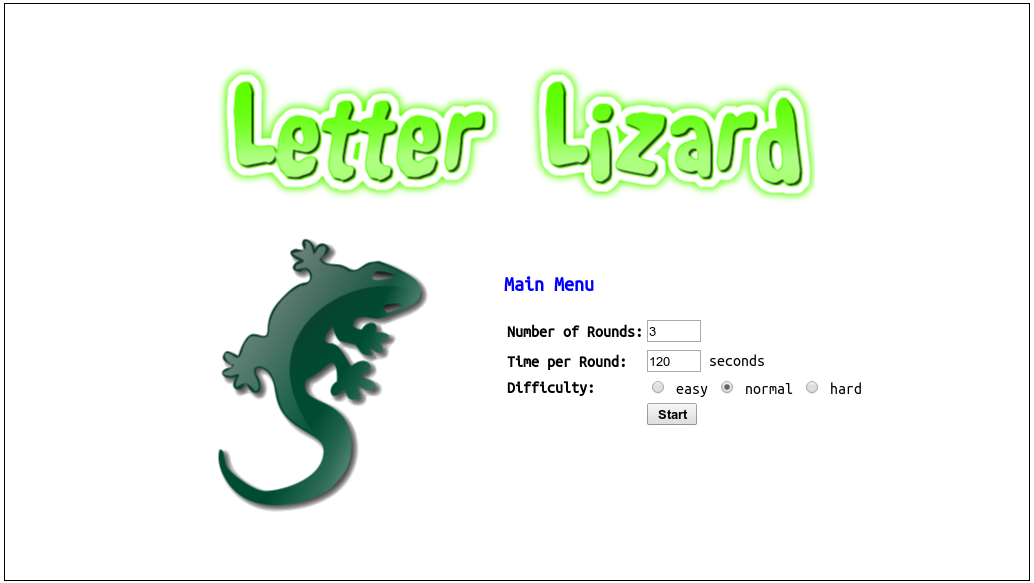
\includegraphics[width=0.9\textwidth]{../screenshots/LetterLizardJS-MainMenu2.png}
        \caption{Main Menu}
        \label{lljsmm}
    \end{subfigure}
    \begin{subfigure}{0.49\textwidth}
        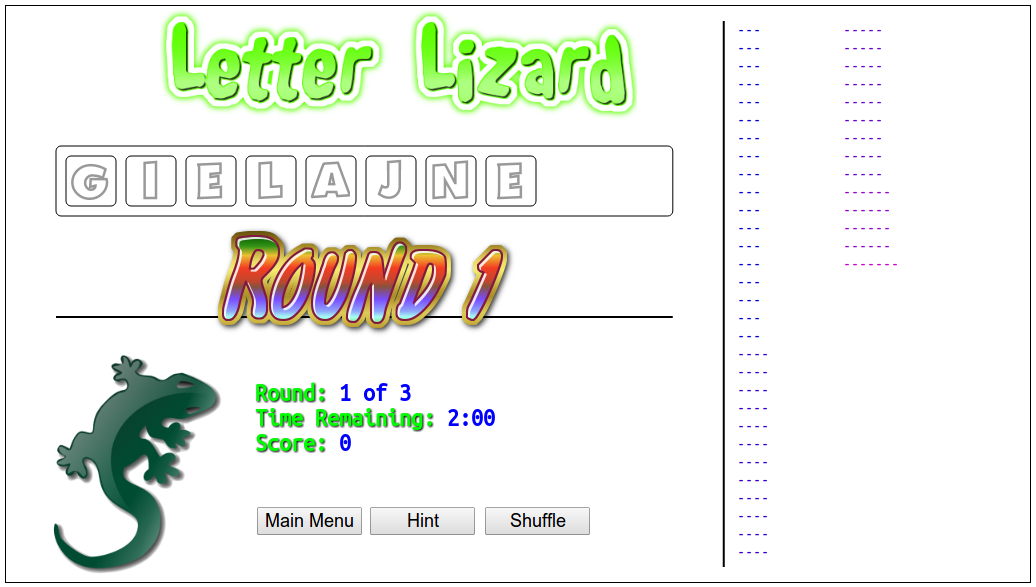
\includegraphics[width=0.9\textwidth]{../screenshots/LetterLizardJS-Round1.png}
        \caption{Round Number message}
        \label{lljsround}
    \end{subfigure}
    \begin{subfigure}{0.49\textwidth}
        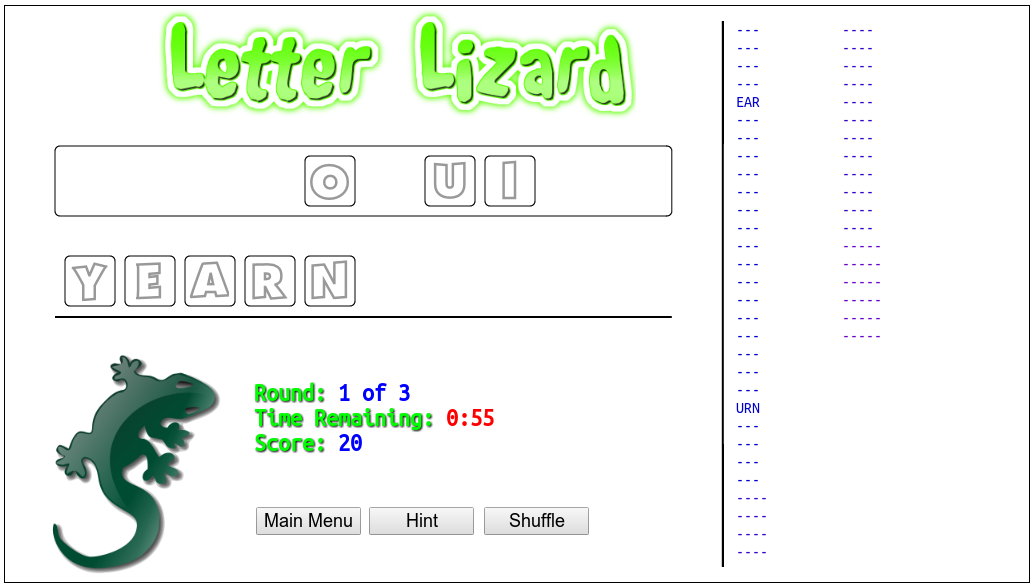
\includegraphics[width=0.9\textwidth]{../screenshots/LetterLizardJS-Gameplay2.png}
        \caption{Game Screen}
        \label{lljsgame}
    \end{subfigure}    
    \begin{subfigure}{0.49\textwidth}
        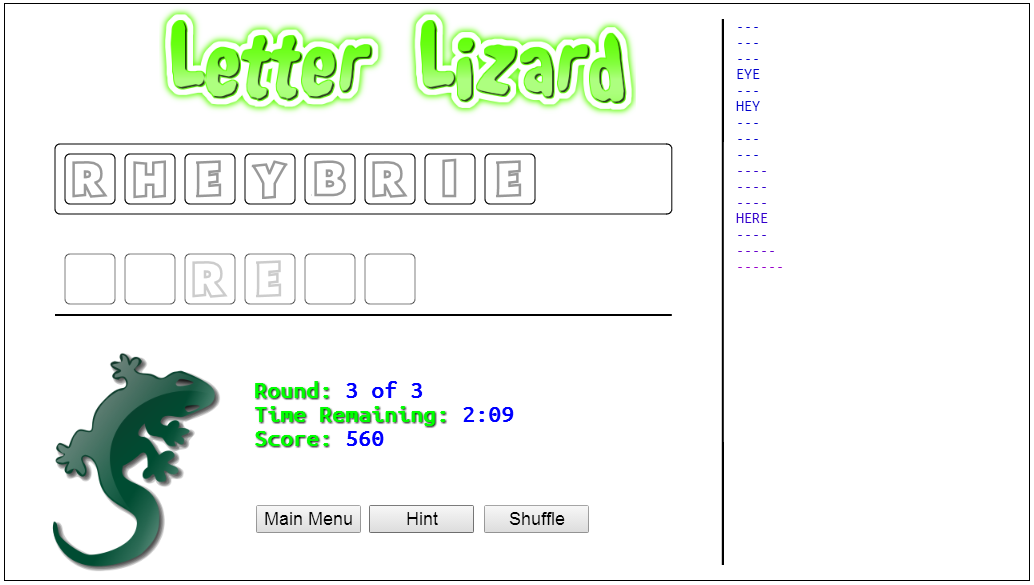
\includegraphics[width=0.9\textwidth]{../screenshots/LetterLizardJS-Hint2.png}
        \caption{Hint}
        \label{lljshint}
    \end{subfigure}
    \begin{subfigure}{0.49\textwidth}
        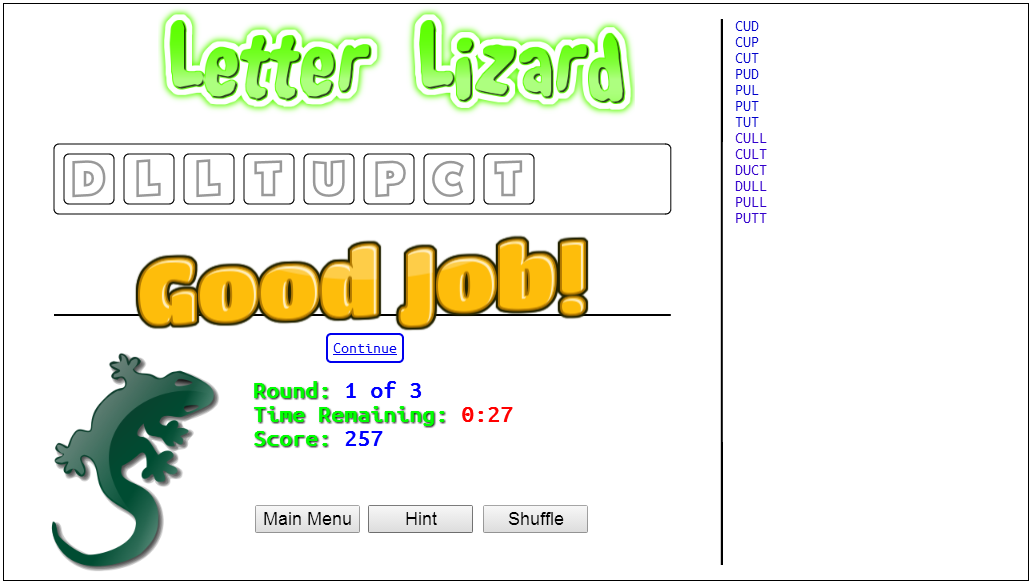
\includegraphics[width=0.9\textwidth]{../screenshots/LetterLizardJS-GoodJob3.png}
        \caption{Good Job message}
        \label{lljsgoodjob}
    \end{subfigure}
    \begin{subfigure}{0.49\textwidth}
        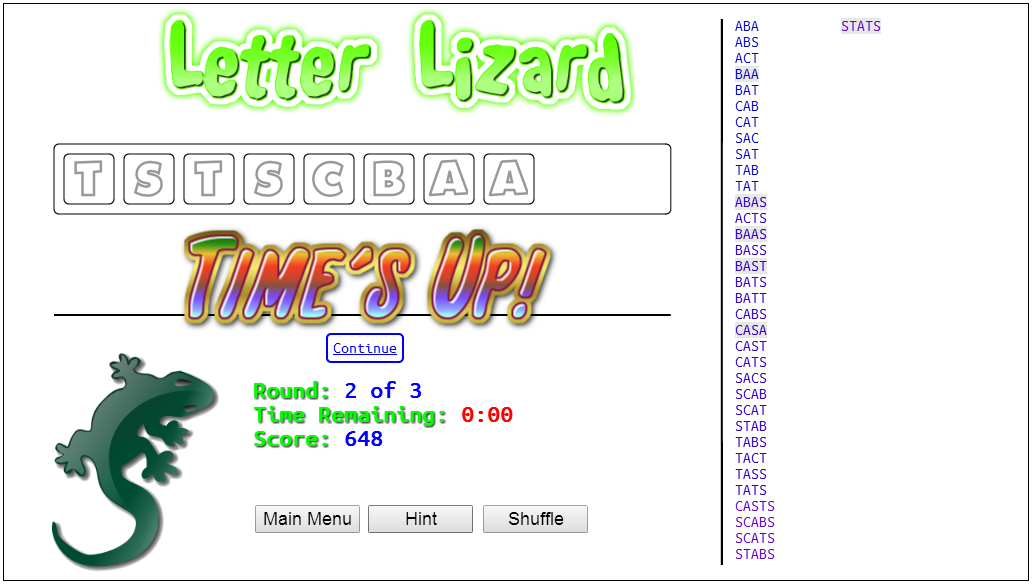
\includegraphics[width=0.9\textwidth]{../screenshots/LetterLizardJS-TimesUp.png}
        \caption{Time's Up message}
        \label{lljstimeup}
    \end{subfigure}
    \begin{subfigure}{0.49\textwidth}
        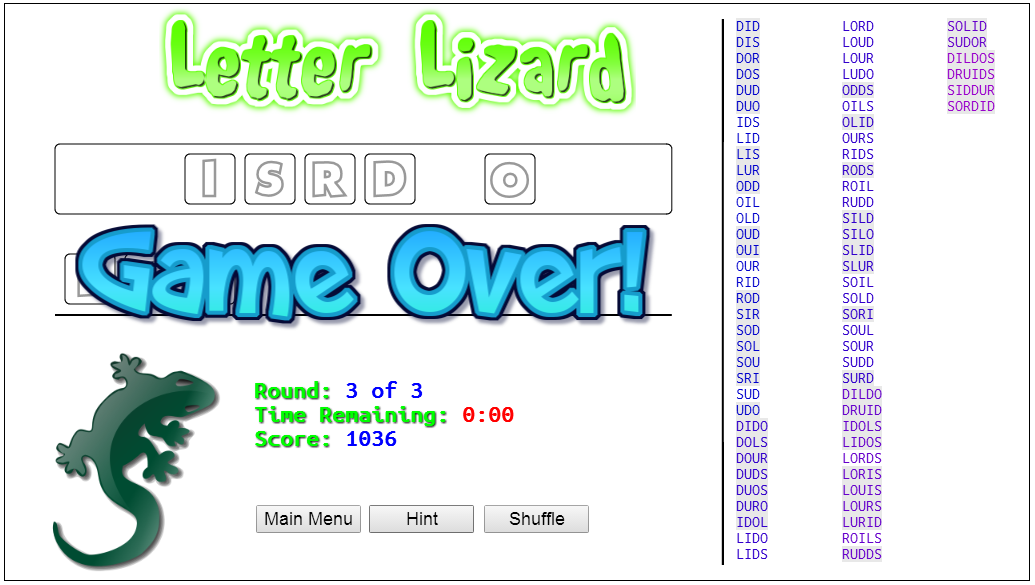
\includegraphics[width=0.9\textwidth]{../screenshots/LetterLizardJS-GameOver2.png}
        \caption{Game Over message}
        \label{lljsgameover}
    \end{subfigure}
    \caption[Screenshots from the Letter Lizard JavaScript implementation]
    {Screenshots from the Letter Lizard JavaScript implementation showing
    (a) the splash screen, (b) the main menu, (c) a round number message that is 
    displayed at the start of each round, (d) the main game screen as a user plays
    the game, (e) an in-game hint, (f) the ``Good Job!'' message that is displayed when
    a player finds all of the words, (g) the ``Time's Up!'' message that is displayed
    when the user does not find all of the words before the time runs out, and (h)
    the ``Game Over!'' message displayed at the end of the game.}
    \label{lljsscreenshots}
\end{figure}

Figure~\ref{lljsscreenshots} shows eight screenshots from LetterLizardJS. When the player
opens the Letter Lizard game in their browser, they are shown the Splash Screen
(Figure~\ref{lljssplash}) that provides information about the game and prompted to
press the space bar to continue. After pressing the space bar, the player is presented
with the Main Menu (Figure~\ref{lljsmm}) that allows them to set the game options, namely
the number of rounds, time per round and level of difficulty. Once the game starts,
the player is presented with a set of letters represented as tiles on the game screen.
The player can move the tiles to form words by typing on the keyboard (Figure~\ref{lljsgame}).
At any time while playing the game, the player can get help to find additional words
by pressing the space bar or clicking the \textbf{Shuffle} button to shuffle the letters,
or by requesting a hint by clicking the \textbf{Hint} button (Figure~\ref{lljshint}).
A number of in-game message are displayed to the user while the game is being played,
which are shown in Figures~\ref{lljsround} and \ref{lljsgoodjob}-\ref{lljsgameover}.

\begin{figure}
    \centering
	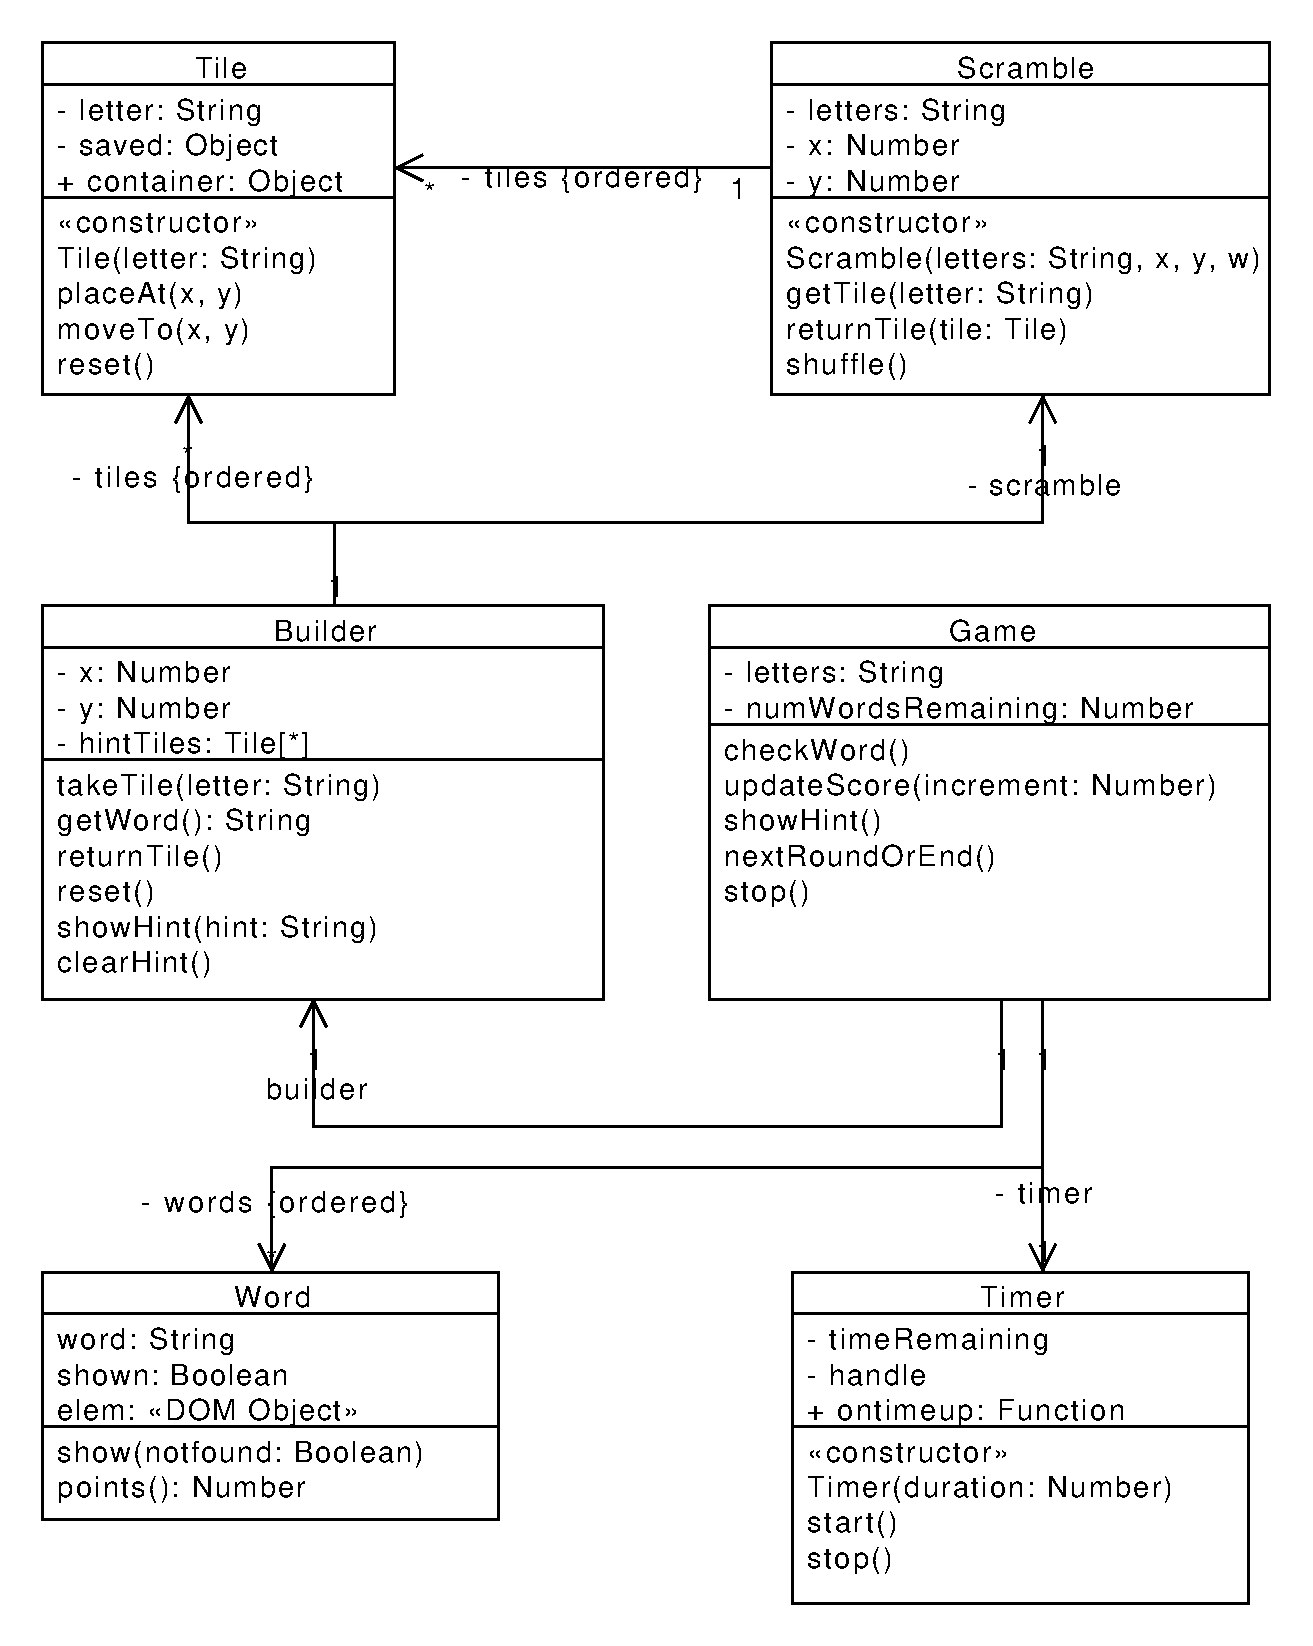
\includegraphics[scale=0.6]{../diagrams/LetterLizardJS-ClassDiagram.pdf}
	\caption[A class diagram for LetterLizardJS]{A class diagram showing the classes that make up the Letter
	Lizard JavaScript implementation. The event-driven, callback-based client-side scripting
	environment naturally led to a modularized, class-based design for this implementation.}
	\label{lljsclasses}
\end{figure}

\begin{figure}
    \centering
	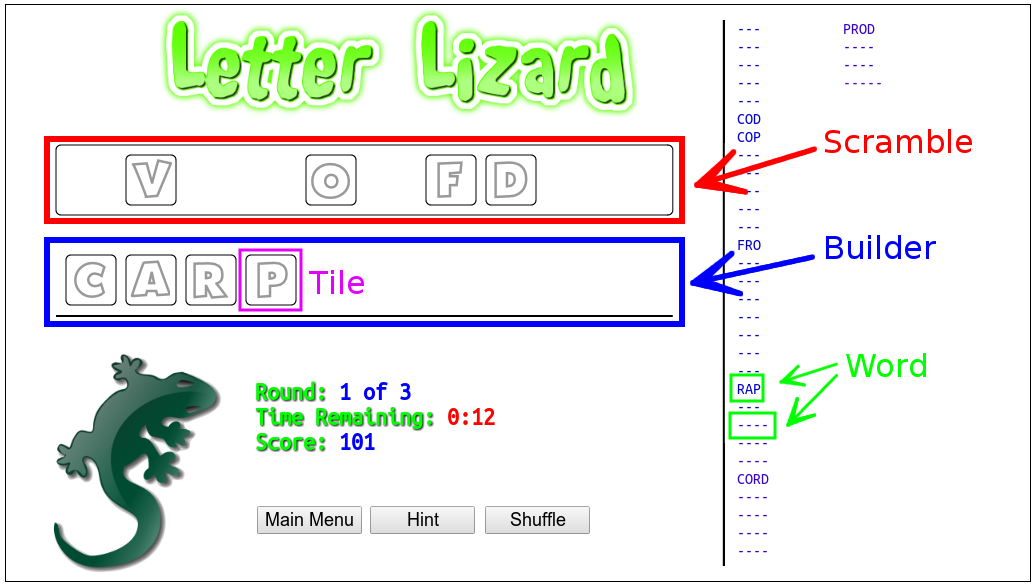
\includegraphics[width=\textwidth]{../screenshots/LetterLizardJS-Legend.png}
	\caption{The on-screen representation of the Scramble, Builder, Tile and Word
	classes.}
	\label{lljslegend}
\end{figure}

One of the main differences that we first noticed between Python, Lua and 
JavaScript had to do with the event-driven nature of the client-side scripting
environment rather than the language itself: at the core of the the Python implementation
is a game loop that processes events and redraws the screen. The Lua implementation does 
not have a game loop like Python, but it still has an update function that draws every
frame of the game to the screen, whereas the JavaScript version does not have any such 
construct. Rather, the JavaScript version is entirely event driven. 
The game loop and update functions Python and Lua naturally led to a
more procedural-based design, but the event-driven JavaScript environment
naturally led to a more modular, object-oriented design. Most of the functionality
of LetterLizardJS is implemented by the six classes shown in Figure~\ref{lljsclasses}.
The Tile, Scrabmle, Builder and Word classes also draw themselves on the main
game screen and their on-screen representation is shown in Figure~\ref{lljslegend}.
The Scramble class is responsible for creating Tiles for the letters that
will be shown to the user and initially places those tiles on itself on the
game screen. It also provides a shuffle method to rearrange the tiles when requested.
The Builder class moves the Tiles to form words when the user types on the keyboard
and also displays hints. The Game class is responsible for creating Word objects
to represent words to be found. It also gets the characters that the user has typed
from the Builder class and checks to see if they are valid words. If so, it causes
the corresponding Word object to show itself in the word list. The
Game class also updates the player's score when they find a word and manages
the game timer.

The code for our JavaScript implementation can be found in our Github repository
(\texttt{uwaterloo-cs798scripting / group4}) under the LetterLizardJS folder. To play the
game, you simply need to load the \texttt{index.html} file in your browser; however,
due to the security policies of most Web browsers that restrict the functionality
of scripts loaded as local files, you will likely have to run an
HTTP server on your local machine and load the \texttt{index.html} file through
your server in order to play the game. Alternatively, we invite you to play the
game using a server that we have set up at using the following URL: 
\url{http://dahu.in/static/LetterLizardJS/index.html}.
